% This is samplepaper.tex, a sample chapter demonstrating the
% LLNCS macro package for Springer Computer Science proceedings;
% Version 2.21 of 2022/01/12
%
\documentclass[runningheads]{llncs}
%
\usepackage[T1]{fontenc}
% T1 fonts will be used to generate the final print and online PDFs,
% so please use T1 fonts in your manuscript whenever possible.
% Other font encondings may result in incorrect characters.
%
\usepackage{graphicx}
% Used for displaying a sample figure. If possible, figure files should
% be included in EPS format.
%
% If you use the hyperref package, please uncomment the following two lines
% to display URLs in blue roman font according to Springer's eBook style:
%\usepackage{color}
%\renewcommand\UrlFont{\color{blue}\rmfamily}
%\urlstyle{rm}
%
 \usepackage{hyperref}
\begin{document}

%\titlerunning{Abbreviated paper title}
% If the paper title is too long for the running head, you can set
% an abbreviated paper title here


\title{MPDW Project Report - Phase 1}
\author{David Castro\inst{1,2} \and
Yaroslav Hayduk\inst{1,3} \and
Bruno Baptista\inst{1,4}}
%
% First names are abbreviated in the running head.
% If there are more than two authors, 'et al.' is used.
%
\institute{FCT UNL, Department of Computer Science \and
60973, djc.castro@campus.fct.unl.pt \and
60739, y.hayduk@campus.fct.unl.pt \and
59815, bm.baptista@campus.fct.unl.pt
}
%
\maketitle              % typeset the header of the contribution
%
%\begin{abstract}


%\keywords{First keyword  \and Second keyword \and Another keyword.}
%\end{abstract}
%
%
%
\vspace{2\baselineskip} % space sections out

\section{Introduction}
This project addresses the challenge of semantic video moment retrieval using transformer-based architectures. The goal is to create a system that can understand user queries and retrieve temporally relevant segments ("video moments") from long videos.

In phase 1, we focused on understanding and building embedding spaces, indexing video captions, and enabling semantic search using dual encoders and OpenSearch. This involved parsing the \href{https://huggingface.co/datasets/HuggingFaceM4/ActivitiyNet_Captions}{ActivityNet Captions dataset} (used as our base for video content and metadata), selecting key videos and processing their moments, extracting representative keyframes, computing both textual and visual embeddings, and indexing and querying the data using OpenSearch with support for k-nearest-neighbor search.

\vspace{2\baselineskip} % space sections out

\section{Algorithms and Implementation}
The system is built on a modular pipeline that prepares video data and metadata for indexing and retrieval using dual encoder architecture. The key components of this implementation include:

\begin{itemize}
    \item Video moment selection and parsing,
    \item Frame extraction and keyframe identification,
    \item Dual encoder embedding generation (text and vision),
    \item OpenSearch index creation and document ingestion,
    \item Search using text and embedding vectors (semantic search).
\end{itemize}

\subsection{Embedding Representations}
We employed a dual encoder approach using the following pre-trained models:

\begin{itemize}
    \item \textbf{Textual Embeddings:} Generated using the sentence-transformers/all-mpnet-base-v2 model from HuggingFace. Captions were tokenized and passed through the transformer model. We applied mean pooling across token embeddings to obtain a 768-dimensional sentence vector for each video caption.
    \item 
    \item \textbf{Visual Embeddings:} Generated for extracted keyframes using the ViT-B-32 variant of CLIP, loaded through open\_clip. Images were preprocessed and encoded using the CLIP image encoder. The resulting 512-dimensional vectors were normalized.
\end{itemize}

Each document in our OpenSearch index represents a keyframe extracted from a video. If the timestamp of a keyframe falls within the range of a moment's start and end time, a document is indexed for that (keyframe, moment) pair. As a result, the same keyframe can appear in multiple documents if it belongs to multiple overlapping moments. Each document includes metadata such as the video ID, moment timestamps, caption, keyframe image path, and their respective embeddings computed using MPNet(for text) and CLIP(for image).

\paragraph{Contextual embeddings:}For visualizing contextual embeddings, we utilized the caption of one of our videos: "A man is in a skateboard track, then he throws a bowling ball that goes around and hits the pins.". The resulting graphs of the layers zero to eleven can be seen in Fig.~\ref{hidden_layers}.

\begin{figure}
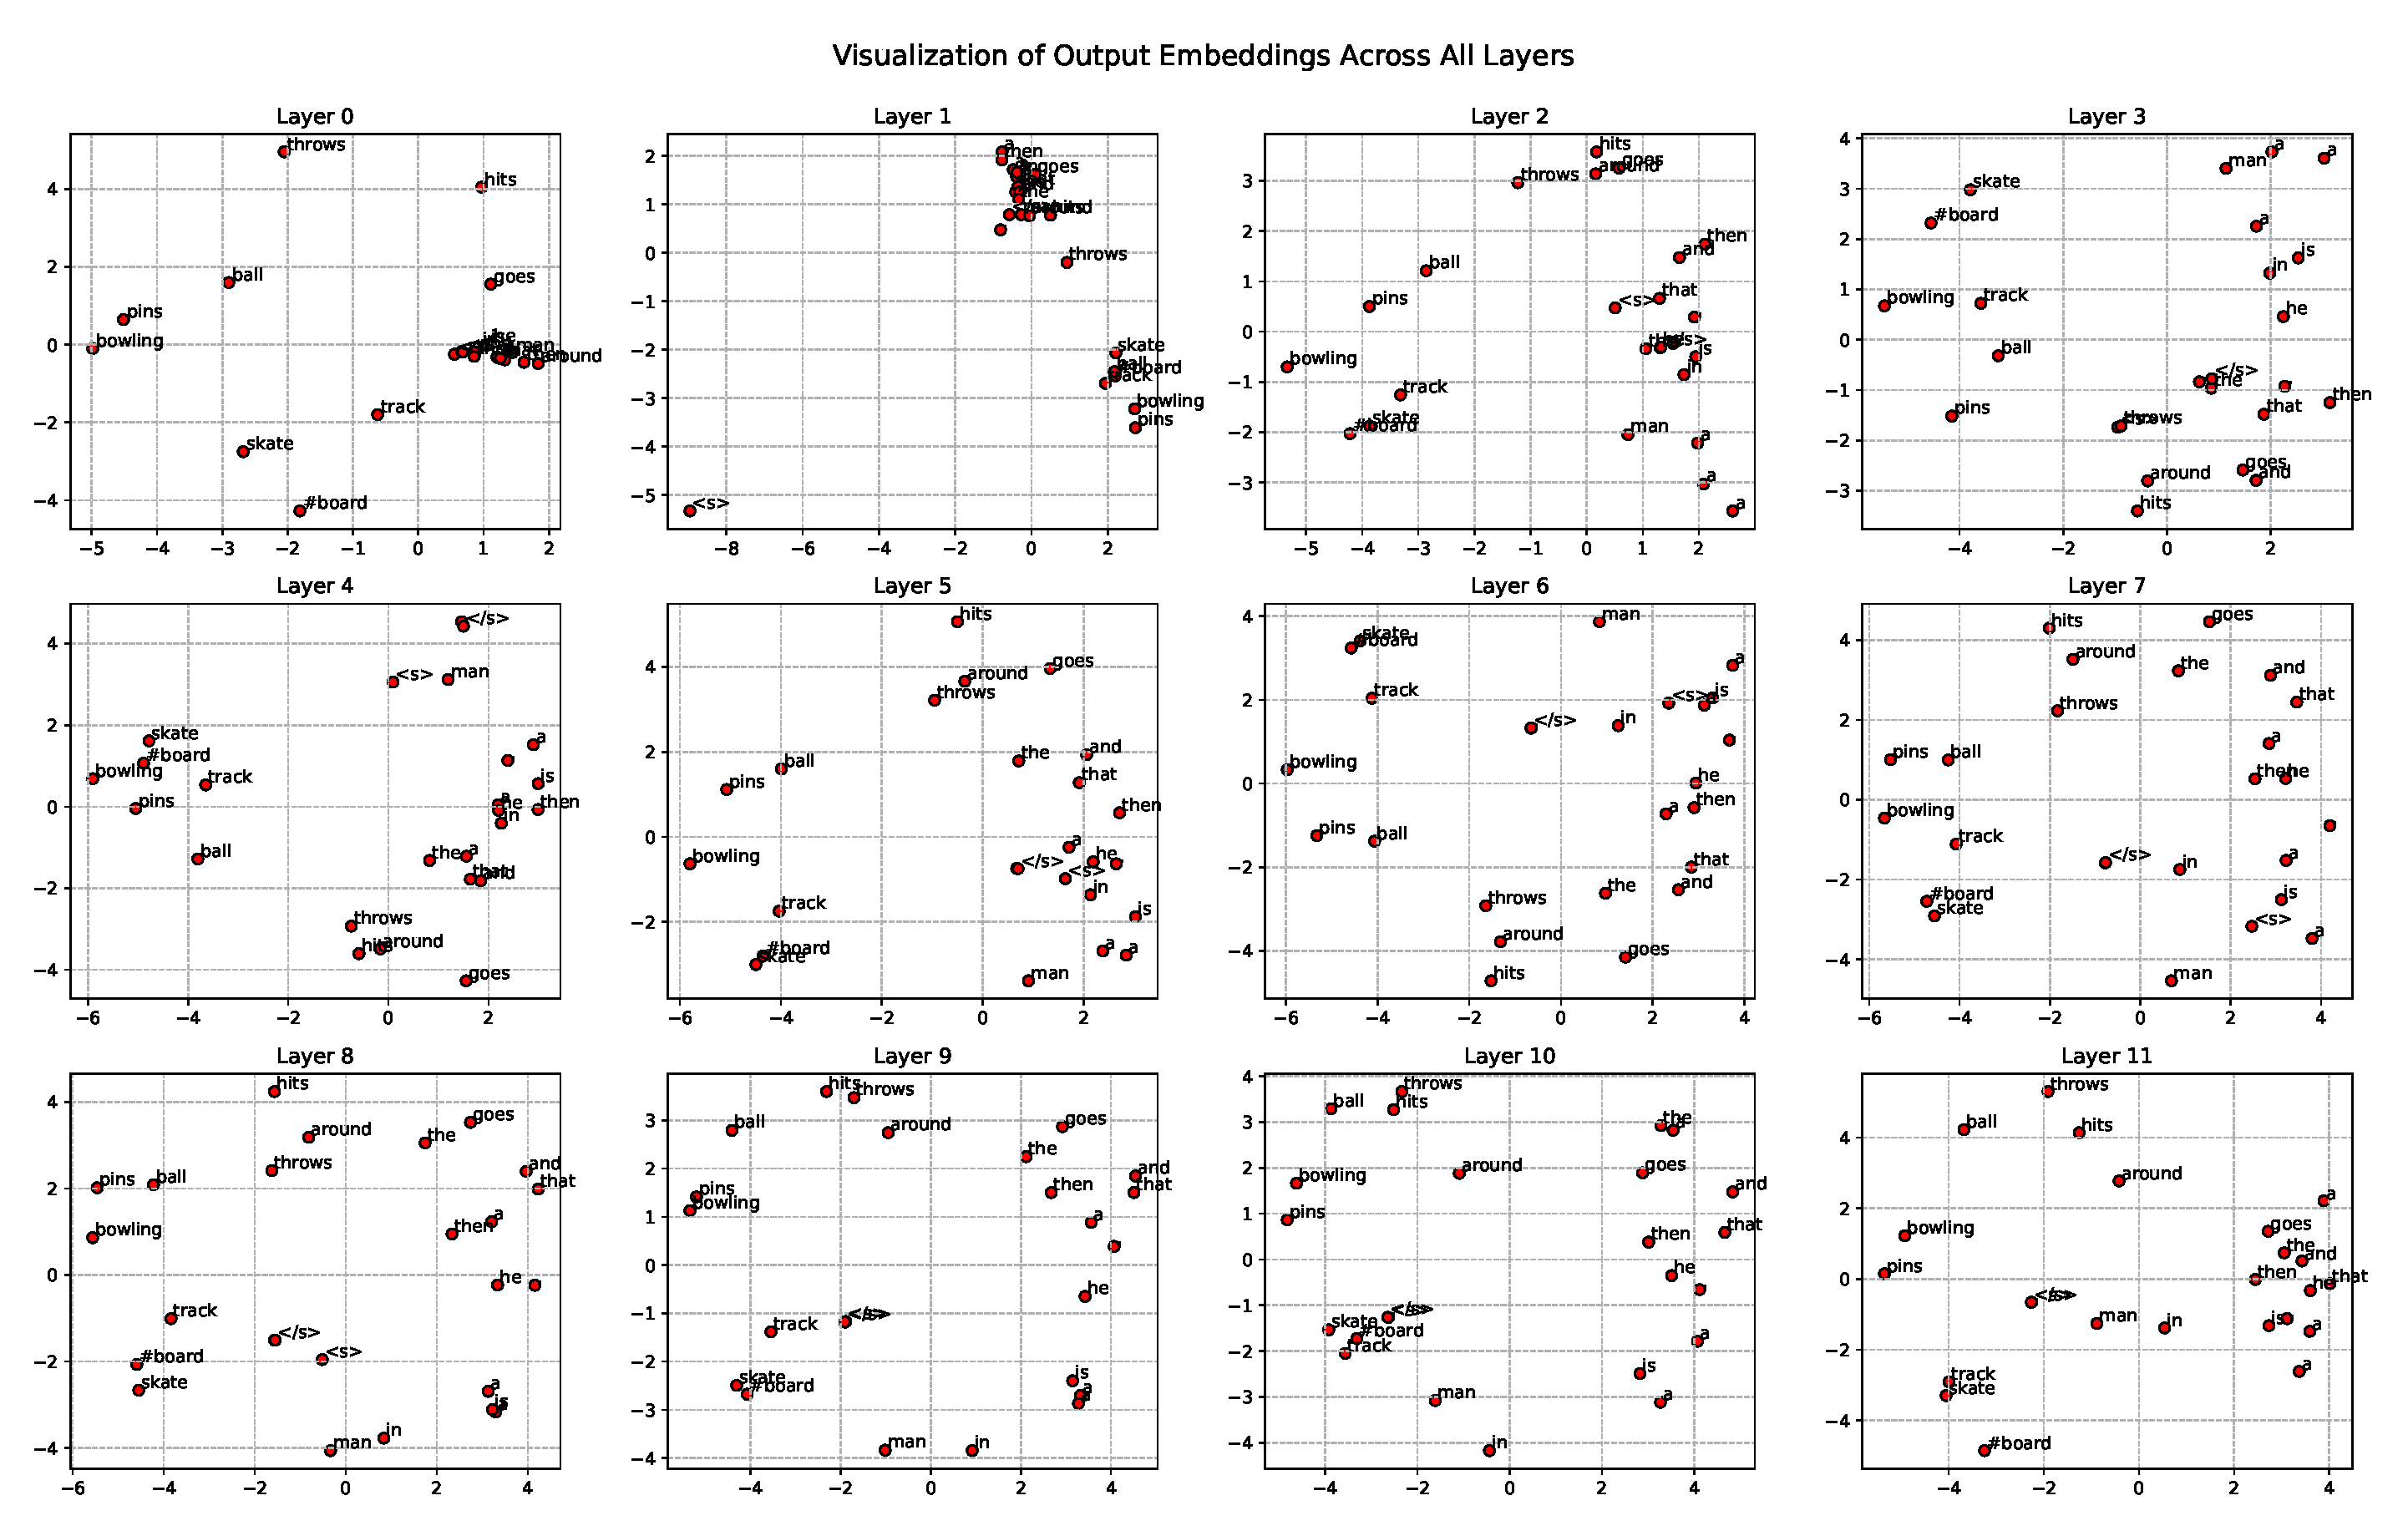
\includegraphics[width=\textwidth]{hidden_layers.eps}
\caption{Contextual embeddings} \label{hidden_layers}
\end{figure}

Surprisingly, in the first layer, the embeddings are very similar to their values in the eleventh layer, but this outcome is merely coincidental, while in the second layer we get something that would be more expected, that is, most embeddings are fairly close together with seemingly no relation or logic. With the progression of the layers, we can see the embeddings disperse and form sensible groups. Namely, we can see the terms "bowling" and "pins" very close together and far from most other words. This makes sense given how specific and relatively rare those words are. The same can be observed for skate, track and board - the suffix of skateboard, hence the proximity. Lastly, the most obvious cluster, on the right: the most common english words. Words such as "a", "the", "that" and "and" which, due to the frequent and indiscriminate use that is given to them, hold very little semantic value and weight in the meaning of sentences.

\paragraph{Positional embeddings:}By repeating the previous exercise with a sentence of the same word repeated 20 times instead, what we get is the positional embeddings of our sentence (see Fig.~\ref{pos_embeds}). The result is a phenomenon that can be explained by the gradual decrease of positional importance throughout the sentence. Stated in simpler terms, the farther a token is from the first word, the smaller the importance of its position. The first word is the one we can see down at the bottom, the farthest from all the others, as its position has the highest relevance. As we move forth in the sentence, the position relevance gradually decreases and we get increasingly similar embeddings. Due to this, we see the converging effect that results in the cluster of points we see at the top, with all the embeddings of the last words close together.

\begin{figure}
  \centering
  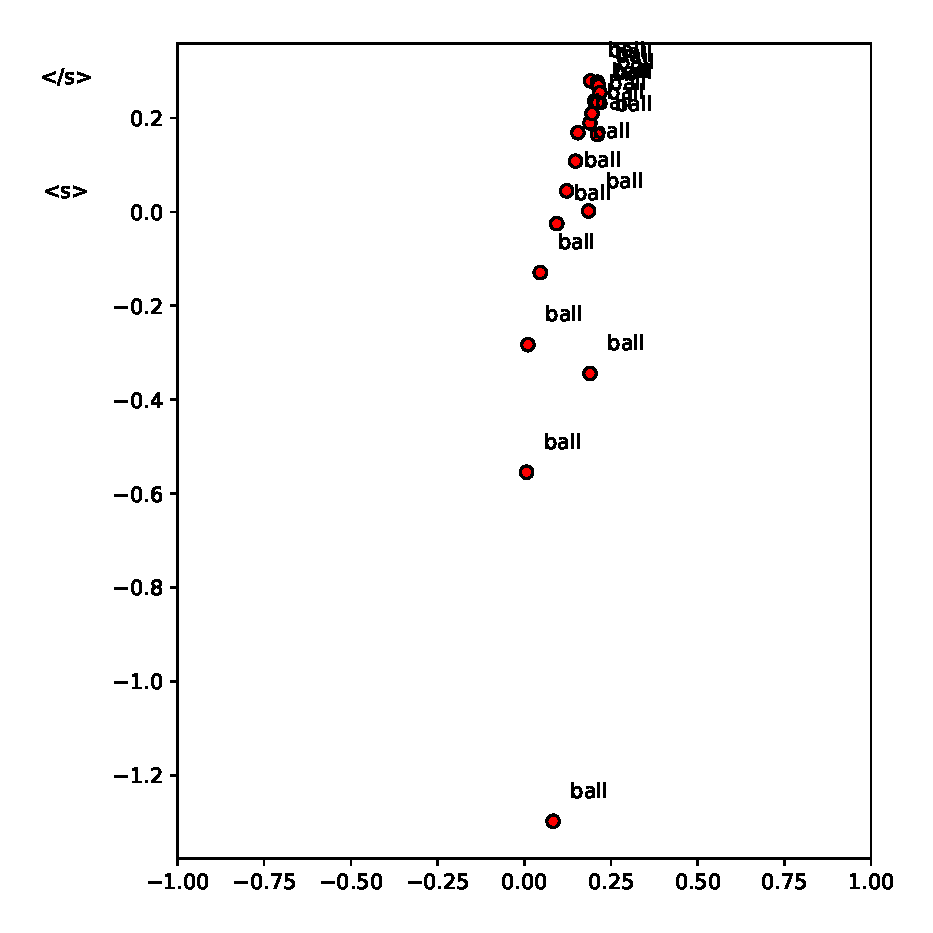
\includegraphics[width=.5\textwidth, clip=true, trim = 15mm 0mm 0mm 0mm]{pos_embeds.eps}
  \caption{Positional embeddings} \label{pos_embeds}
  \label{img:positional_embeddings}
\end{figure}

\subsection{Large Vision and Language Models}
While Phase 2 will delve deeper into large vision and language models, in Phase 1 we already used pretrained transformers:

\begin{itemize}
    \item \textbf{MPNet (All-MPNet-Base-V2)} for generating context-aware text embeddings.
    \item \textbf{CLIP (ViT-B/32)} to embed keyframes into a multimodal representation space.
\end{itemize}

These models enable semantic alignment between visual content and natural language descriptions.

\subsection{Attention}

\begin{figure}
  \centering
  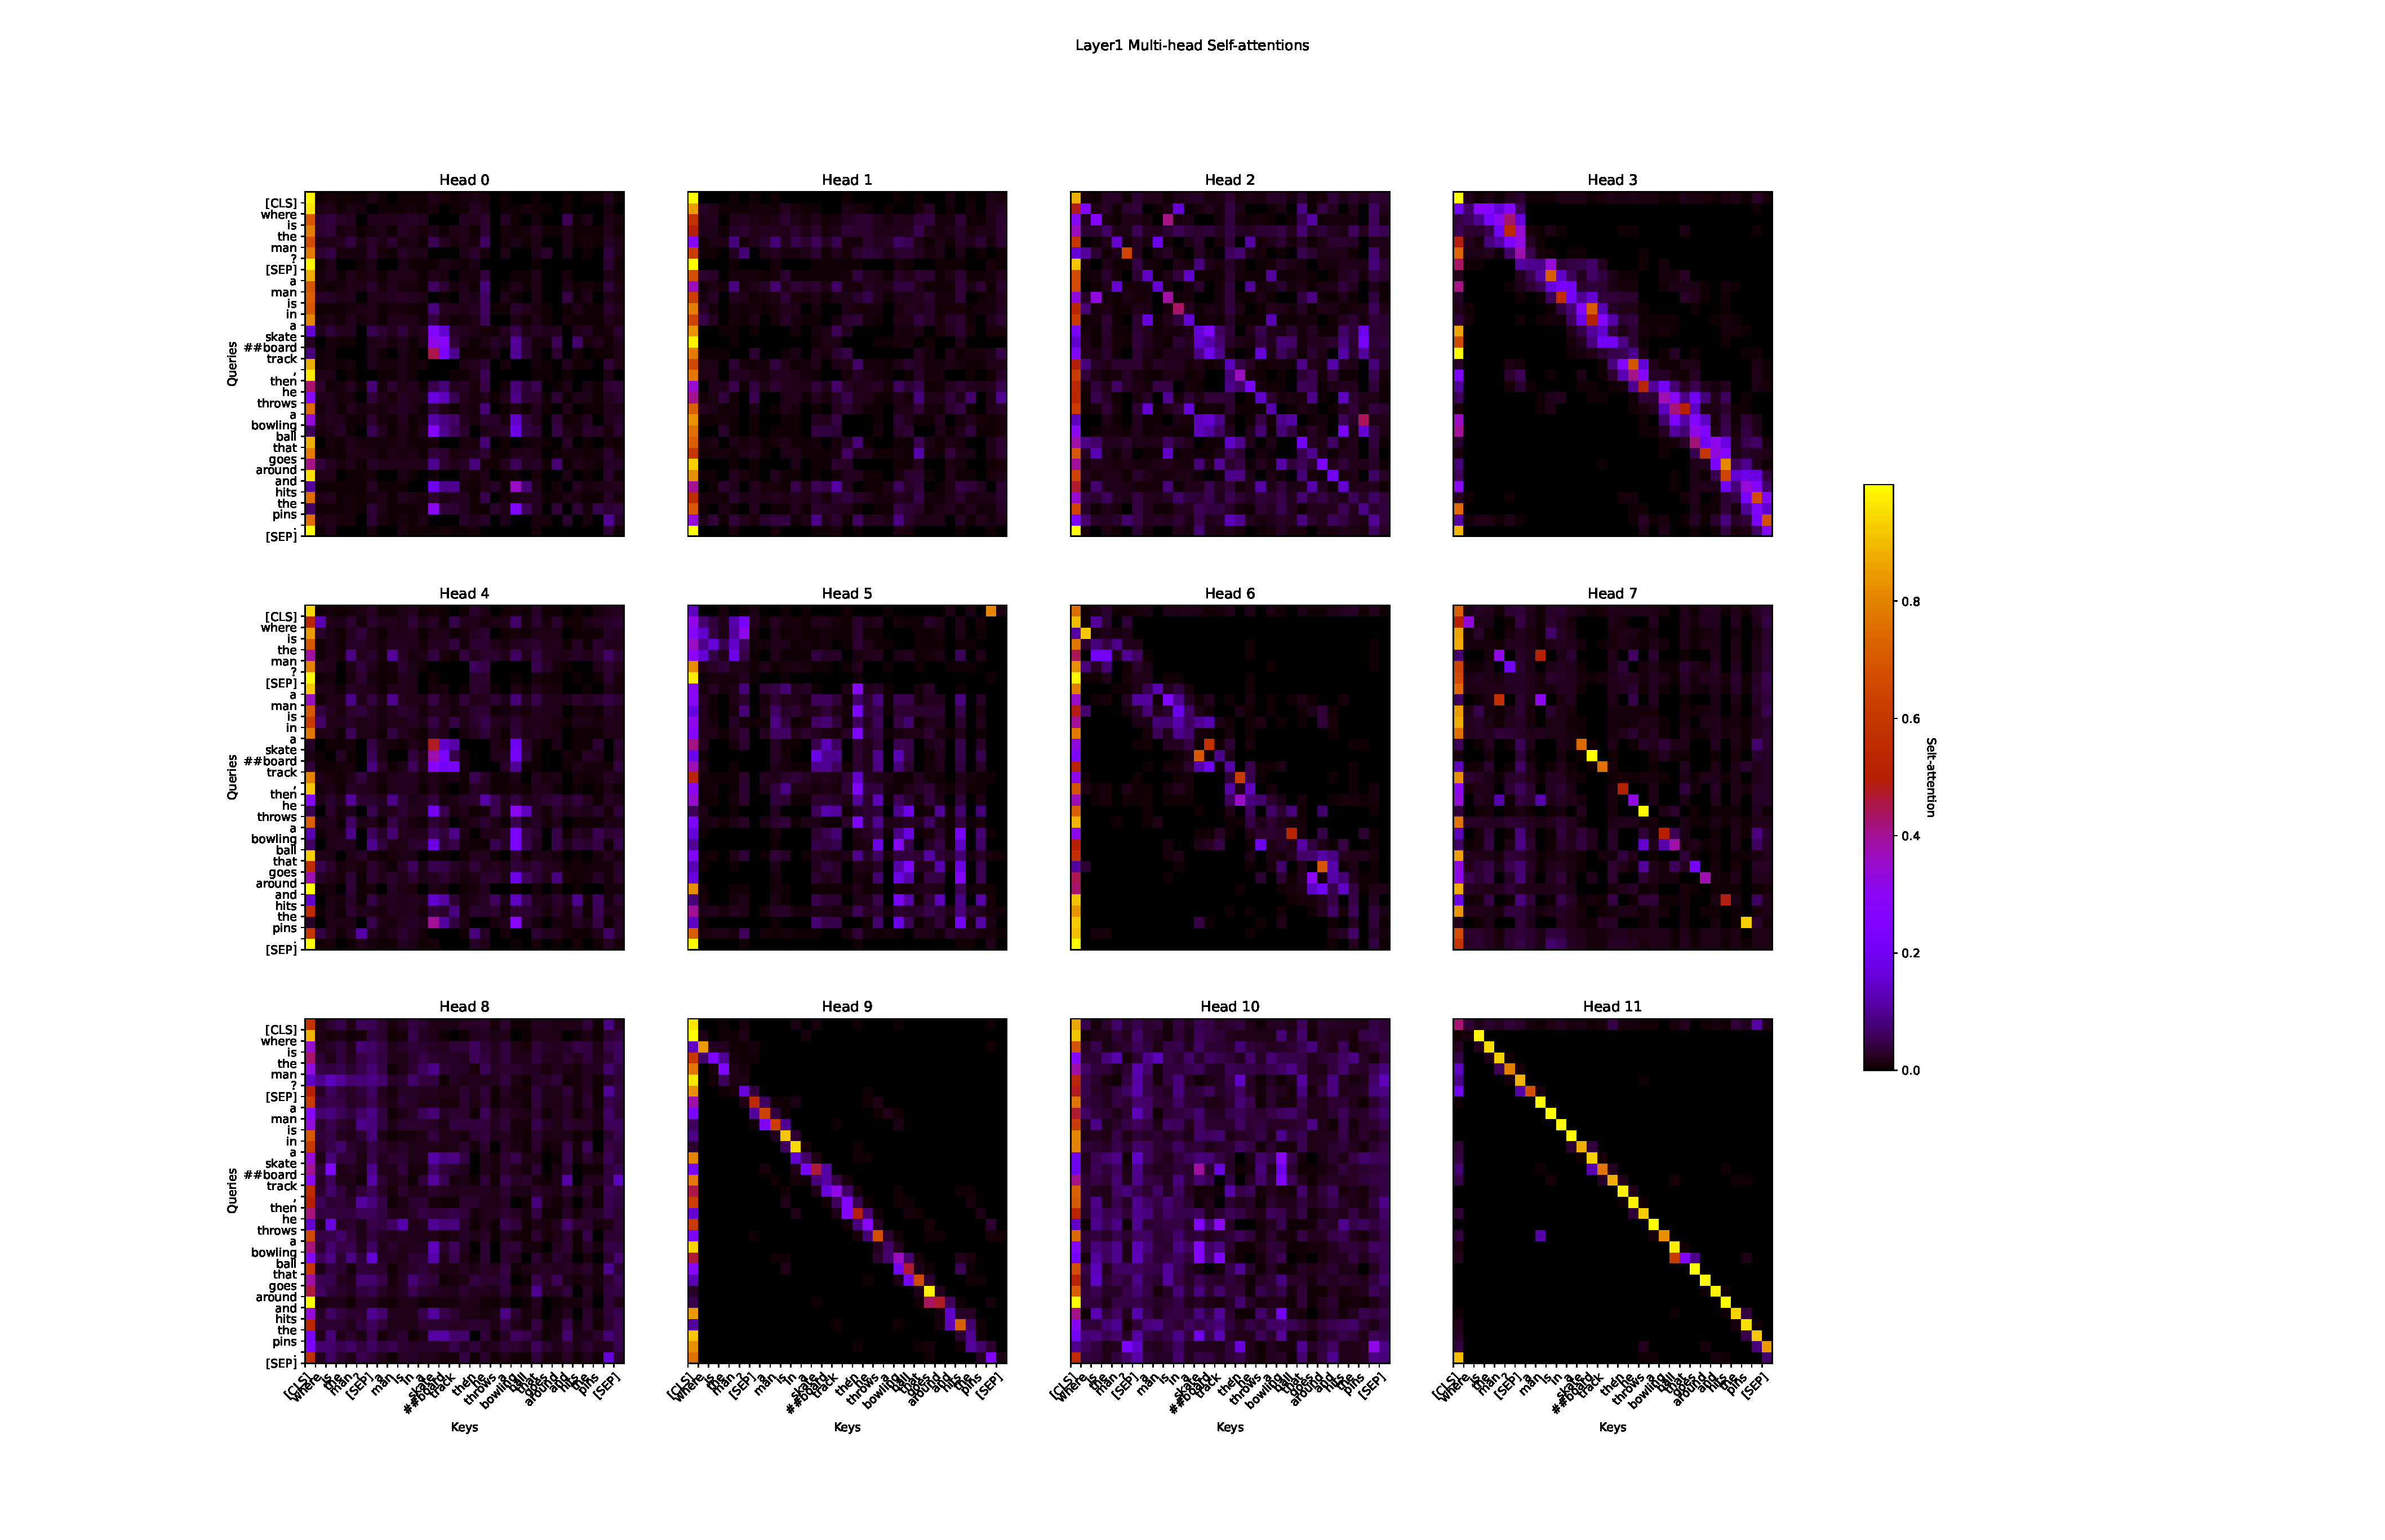
\includegraphics[width=\textwidth, clip=true, trim = 70mm 25mm 130mm 45mm]{self_att_heads.eps}
  \caption{Self-attention} \label{self_att_heads}
  \label{img:self_attention}
\end{figure}

\paragraph{Self-attention for Cross-Encoder:} To analyze the model's self-attention mechanism we generated every head's self-attention for the input "where is the man? A man is in a skateboard track, then he throws a bowling ball that goes around and hits the pins.". When looking at the different heads there are multiple patterns we can identify, giving us an intuition of their purpose. A lot of them also simply pay a general, overall attention to the whole sentence. If we look at figure ~\ref{self_att_heads}, head 2 looks at every token relatively the same, with a special interest in itself, given the distinctive diagonal. This phenomenon can be seen even more clearly in head 7. Head 3 shows us a very clear diagonal pattern, where each token pays higher attention to itself and the around 3 to 6 right next to it, with virtually no attention to all the others; this could be loosely interpreted as: this head solely pays attention to the current token and the few right next to it. Similar effects can be seen in other heads, such as head 6, 9 and 11. Head 6 seems to be paying most of its attention to the couple of tokens right before and right after the current token. Head 9 attends pretty much only to the two tokens right behind the current token. While finally, head 11, pays attention almost exclusively to the token immediately after.


\begin{figure}
  \centering
  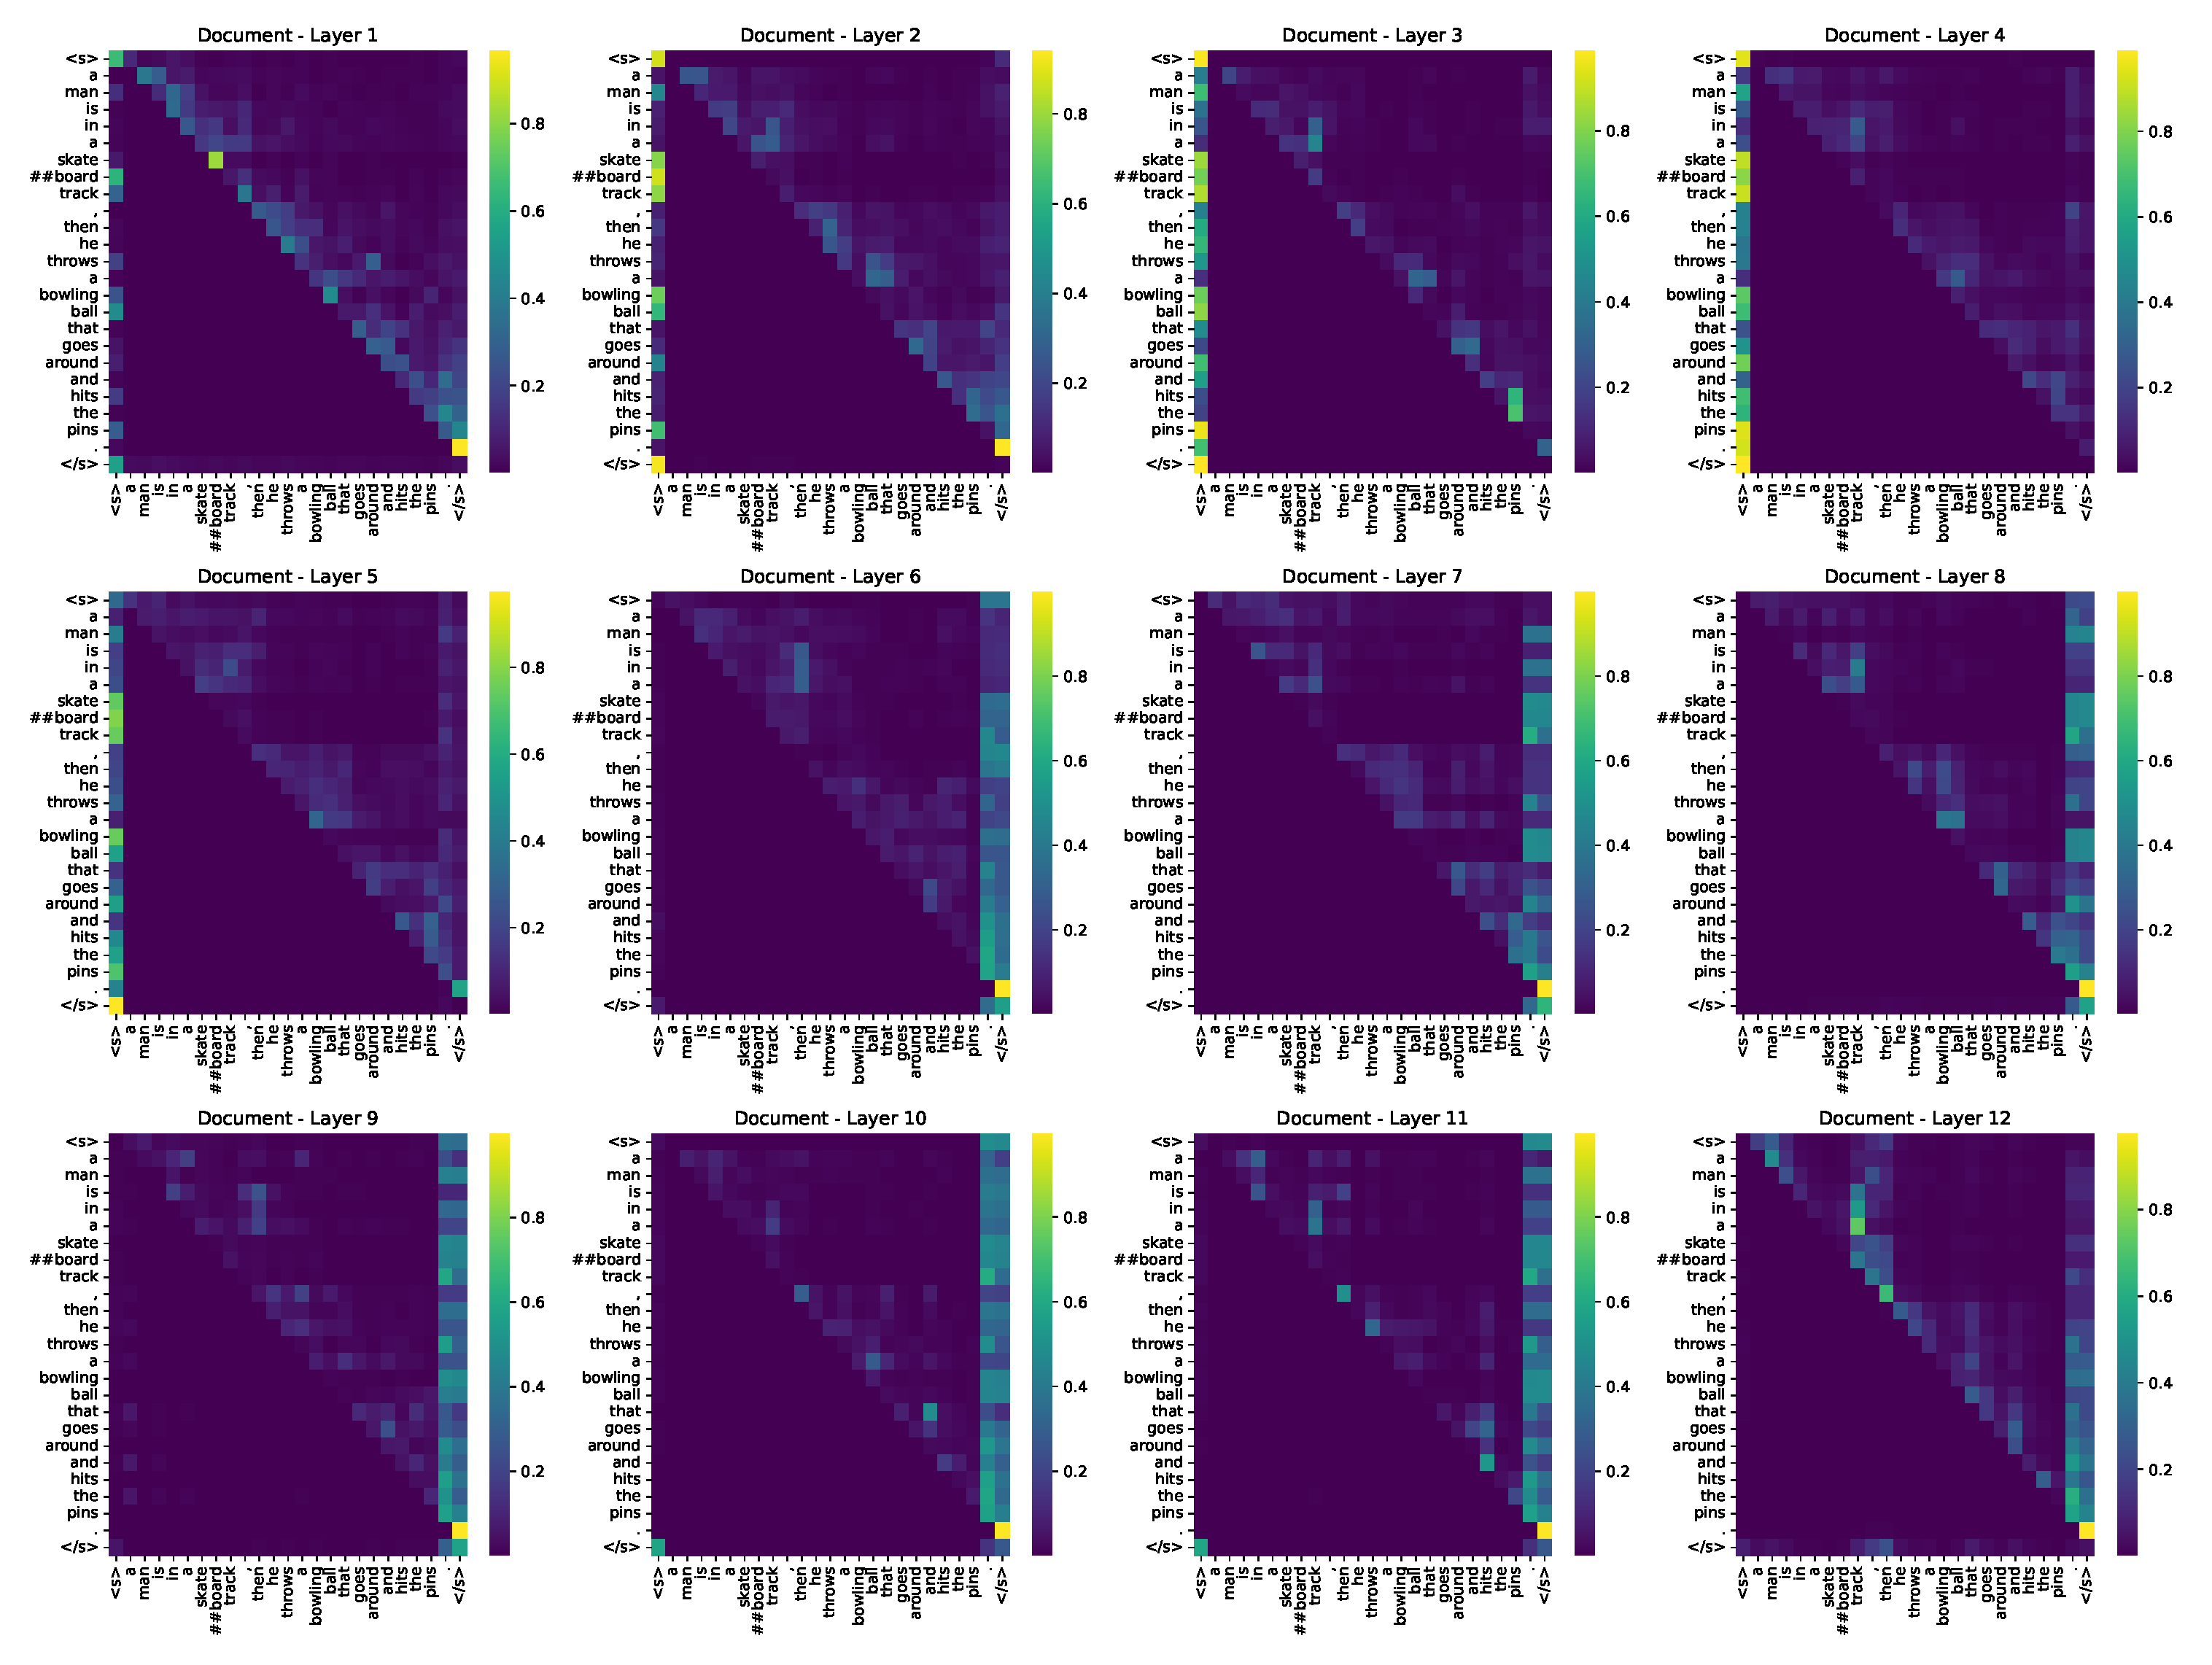
\includegraphics[width=\textwidth, clip=true]{attention_layers_document.eps}
  \caption{Self-attention document} \label{self_att_document}
  \label{img:self_attention_document}
\end{figure}


\begin{figure}
  \centering
  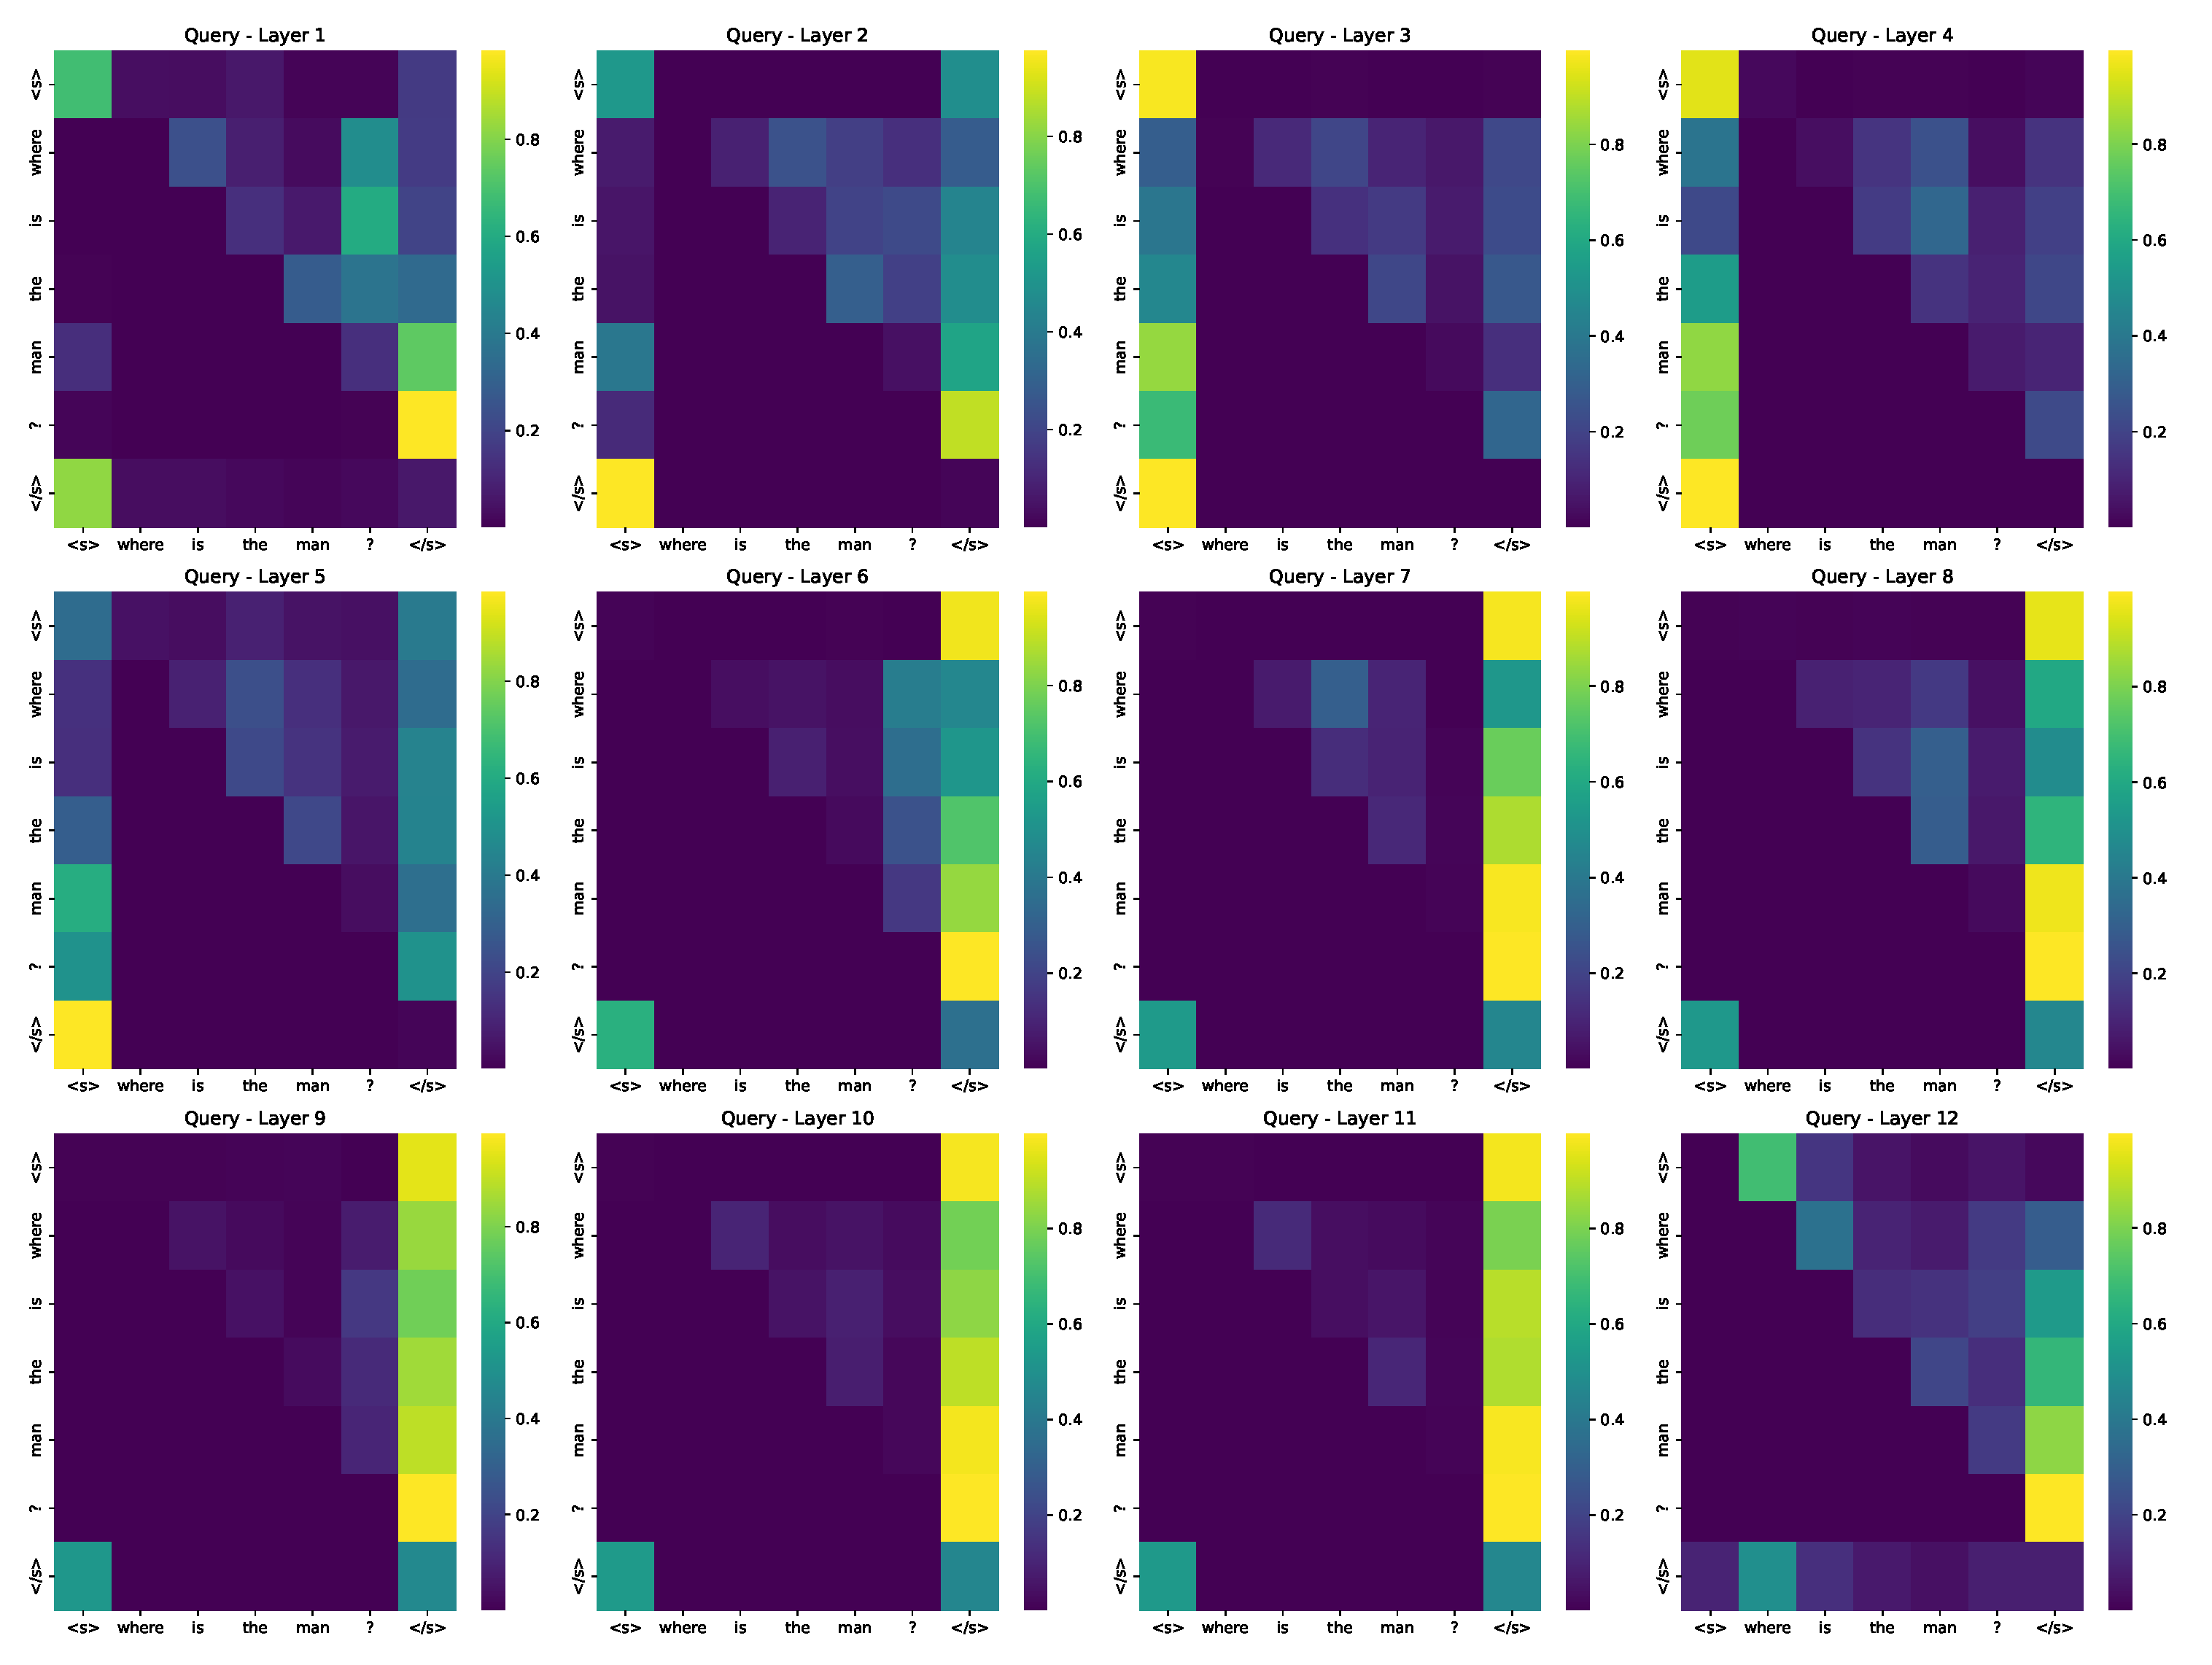
\includegraphics[width=\textwidth, clip=true]{attention_layers_query.eps}
  \caption{Self-attention query} \label{self_att_query}
  \label{img:self_attention_query}
\end{figure}

\paragraph{Self-Attention for Dual-Encoder:} 
In the dual-encoder architecture, the query and document are processed independently, which results in separate self-attention mechanisms for each. To analyze this, we visualized the attention heads for both the query sequence \textit{"Where is the man?"} and the document \textit{"A man is in a skateboard track, then he throws a bowling ball that goes around and hits the pins."}, as shown in Figures~\ref{dual_enc_query} and~\ref{dual_enc_doc}.

For the \textbf{query}, attention patterns are more localized and interpretable due to its short length. Many heads show weak diagonals, indicating that each token attends mostly to those ahead of it. For example, the token \textit{"man"} receives significant self-attention in multiple heads, highlighting its semantic importance in the query. Some heads distribute attention more uniformly across the question, possibly capturing the overall intent.

In contrast, the \textbf{document}'s self-attention shows more diverse behavior. Several heads focus attention across broader spans of the input, capturing syntactic structures or semantic relations within the sentence. For instance, verbs such as \textit{"throws"} or \textit{"hits"} often receive and distribute attention across related nouns like \textit{"ball"} or \textit{"pins"}, suggesting an awareness of action-object relationships. Other heads demonstrate local attention, where each token mainly attends to its immediate neighbors—similar to what is observed in convolutional operations.

Unlike the cross-encoder, the dual-encoder architecture does not allow for query-document token interaction within the attention layers. Instead, it relies on the resulting embeddings of the entire sequences to compute similarity. As such, these self-attention patterns offer insights into how local and global context are captured independently in the query and the document, before any cross-similarity computation is performed.


\vspace{2\baselineskip} % space sections out

\section{Evaluation}

\subsection{Dataset Description}
We used the \href{https://huggingface.co/datasets/HuggingFaceM4/ActivitiyNet_Captions}{ActivityNet Captions dataset}, which provides:

\begin{itemize}
    \item \ensuremath{\sim}20k YouTube videos with natural language descriptions of events,
    \item Timestamp-aligned captions for video moments.
\end{itemize}

In our implementation, we selected from the dataset 10 videos with a reasonable amount of moments. For each:

\begin{itemize}
    \item Keyframes were extracted using PyAV by saving either keyframes or one frame per second.
    \item Corresponding captions were merged and aligned using metadata from three different files: val\_1.json, val\_2.json, and activity\_net.v1-3.min.json.
\end{itemize}

The resulting data was indexed in OpenSearch using custom mappings to support both text-based and embedding-based (knn) search.




%
% ---- Bibliography ----
%
% BibTeX users should specify bibliography style 'splncs04'.
% References will then be sorted and formatted in the correct style.
%
% \bibliographystyle{splncs04}
% \bibliography{mybibliography}
%
\begin{thebibliography}{8}
\bibitem{ref_article1}
Author, F.: Article title. Journal \textbf{2}(5), 99--110 (2016)

\bibitem{ref_lncs1}
Author, F., Author, S.: Title of a proceedings paper. In: Editor,
F., Editor, S. (eds.) CONFERENCE 2016, LNCS, vol. 9999, pp. 1--13.
Springer, Heidelberg (2016). \doi{10.10007/1234567890}

\bibitem{ref_book1}
Author, F., Author, S., Author, T.: Book title. 2nd edn. Publisher,
Location (1999)

\bibitem{ref_proc1}
Author, A.-B.: Contribution title. In: 9th International Proceedings
on Proceedings, pp. 1--2. Publisher, Location (2010)

\bibitem{ref_url1}
LNCS Homepage, \url{http://www.springer.com/lncs}, last accessed 2023/10/25
\end{thebibliography}
\end{document}
